\section{Deep Learning\label{sec:DL}}
%%%%%%%%%%%%%%%%%%%%%%%%%%%%%%%%%%%%%%%%%%%%%%%%%%%%%%%%%%%%%%%%%%%%%%%%%%%%%%%%

\Gls{DL} is a field of \gls{ML} that is primarily concerned with the learning of
representations of data. The main difference between a \gls{NN} and a
traditional \gls{ML} algorithm is that the neural network is a function of the
data, rather than the data itself.

\subsection{Perceptrons}
%%%%%%%%%%%%%%%%%%%%%%%%%%%%%%%%%%%%%%%%%%%%%%%%%%%%%%%%%%%%%%%%%%%%%%%%%%%%%%%%

Proposed by Rosenblatt \cite{Rosenblatt_1957_6098} in his technical
report funded by the United States Office of Naval Research
\cite{doi:10.1177/030631296026003005} in 1957, the \textit{perceptron} is a
fundamental component of deep learning, describing a mathematical model of a
biological neuron. There are two different sets of notation which exist when
dealing with the bias of a perceptron. One involves the inclusion of a unit
constant in the input vector $\mathbf{x}$, with the bias being specified by the
value of the first weight $w_0$. An alternative notation exists which treats the
bias as a standalone value $b$. The latter notation will be used, as it is the
preferred notation in contemporary deep learning research. The notation defining
the mapping of a perceptron is then: $f(\gls{x_in};\gls{w_vec},
\gls{b})=\gls{x_in}^T\gls{w_vec}+\gls{b}$; $\gls{x_in}\in\gls{set:R}^{\gls{n_x}}$,
$\gls{w_vec}\in\gls{set:R}^{\gls{n_x}}$, $\gls{b}\in\gls{set:R}$.

\begin{figure}[htbp]
    \centering
    % MIT License
%
% Copyright (c) 2021 Geoffrey H. Garrett
%
% Permission is hereby granted, free of charge, to any person obtaining a copy
% of this software and associated documentation files (the "Software"), to deal
% in the Software without restriction, including without limitation the rights
% to use, copy, modify, merge, publish, distribute, sublicense, and/or sell
% copies of the Software, and to permit persons to whom the Software is
% furnished to do so, subject to the following conditions:
%
% The above copyright notice and this permission notice shall be included in all
% copies or substantial portions of the Software.
%
% THE SOFTWARE IS PROVIDED "AS IS", WITHOUT WARRANTY OF ANY KIND, EXPRESS OR
% IMPLIED, INCLUDING BUT NOT LIMITED TO THE WARRANTIES OF MERCHANTABILITY,
% FITNESS FOR A PARTICULAR PURPOSE AND NONINFRINGEMENT. IN NO EVENT SHALL THE
% AUTHORS OR COPYRIGHT HOLDERS BE LIABLE FOR ANY CLAIM, DAMAGES OR OTHER
% LIABILITY, WHETHER IN AN ACTION OF CONTRACT, TORT OR OTHERWISE, ARISING FROM,
% OUT OF OR IN CONNECTION WITH THE SOFTWARE OR THE USE OR OTHER DEALINGS IN THE
% SOFTWARE.

%%%%%%%%%%%%%%%%%%%%%%%%%%%%%%%%%%%%%%%%%%%%%%%%%%%%%%%%%%%%%%%%%%%%%%%%%%%%%%%
% ACKNOWLEDGEMENTS
%%%%%%%%%%%%%%%%%%%%%%%%%%%%%%%%%%%%%%%%%%%%%%%%%%%%%%%%%%%%%%%%%%%%%%%%%%%%%%%
% Design and implementation of this diagram was inspired and adapted from:
% https://tex.stackexchange.com/questions/104334/tikz-diagram-of-a-perceptron

%%%%%%%%%%%%%%%%%%%%%%%%%%%%%%%%%%%%%%%%%%%%%%%%%%%%%%%%%%%%%%%%%%%%%%%%%%%%%%%
% DEPENDENCIES
%%%%%%%%%%%%%%%%%%%%%%%%%%%%%%%%%%%%%%%%%%%%%%%%%%%%%%%%%%%%%%%%%%%%%%%%%%%%%%%
%\usepackage{tikz}
%\usetikzlibrary{decorations.pathreplacing}    % for TikZ braces
%\usetikzlibrary{positioning}                  % for TikZ relative positioning

%%%%%%%%%%%%%%%%%%%%%%%%%%%%%%%%%%%%%%%%%%%%%%%%%%%%%%%%%%%%%%%%%%%%%%%%%%%%%%%
% USER STYLING
%%%%%%%%%%%%%%%%%%%%%%%%%%%%%%%%%%%%%%%%%%%%%%%%%%%%%%%%%%%%%%%%%%%%%%%%%%%%%%%

% TikZ node design.
\tikzset{basic/.style={draw,text width=1em,text badly centered}}
\tikzset{input/.style={}}
\tikzset{output/.style={}}
\tikzset{weight/.style={basic,circle}}
\tikzset{hidden/.style={basic,circle}}
\tikzset{function/.style={basic,circle}}

% Labels and symbols.
\def\activationlabel{activation function}  % activation function label
\def\activationsymbol{$\phi$}              % activation function symbol
\def\transferlabel{transfer function}      % transfer function label
\def\transfersymbol{$\sum$}                % transfer function symbol
\def\outputsymbol{$y$}                     % output symbol
\def\inputsymbol{$x$}                      % input symbol
\def\inputvecsymbol{$\mathbf{x}$}          % input vector symbol
\def\weightslabel{weights}                 % input vector symbol
\def\biassymbol{$b$}                       % bias symbol

%%%%%%%%%%%%%%%%%%%%%%%%%%%%%%%%%%%%%%%%%%%%%%%%%%%%%%%%%%%%%%%%%%%%%%%%%%%%%%%
% TIKZ PICTURE
%%%%%%%%%%%%%%%%%%%%%%%%%%%%%%%%%%%%%%%%%%%%%%%%%%%%%%%%%%%%%%%%%%%%%%%%%%%%%%%
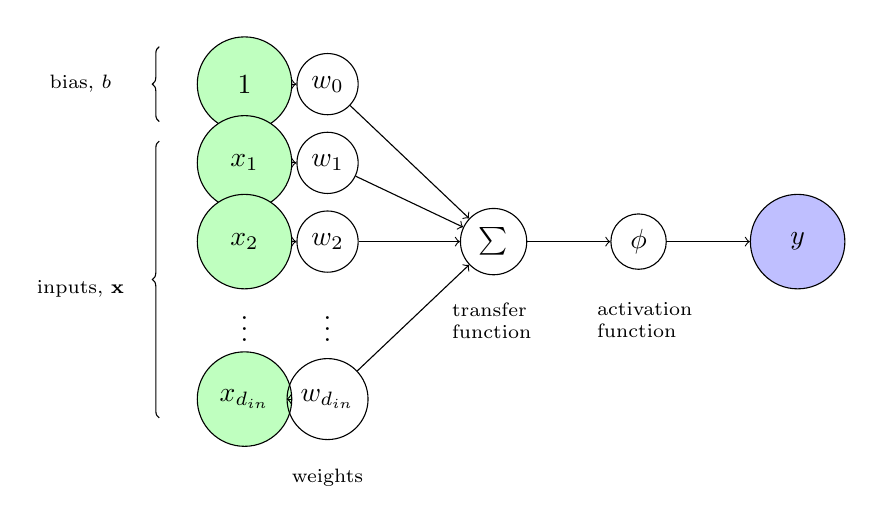
\begin{tikzpicture}
    \node[function] at ({\transferx}, -{int(2)})  (transfer) {\transfersymbol};
    \node[function, right=3em of transfer] (activation) {\activationsymbol};
    \node[below of=activation,font=\scriptsize,text width=3em] {\activationlabel};
    \node[below of=transfer,font=\scriptsize,text width=3em] {\transferlabel};
    \node[output, right=\layersep of activation] (output) {\outputsymbol};
    \path[draw,->] (transfer) -- (activation);
    \path[draw,->] (activation) -- (output);

    % Iterate through each row of units.
    \foreach \n [evaluate=\n as \p using {int(\n-1)}] in {0,1,2,3,4} {
        \ifnum \n=0
        \node[input] at (0, -\n) (X-\n) {$1$};
        \node[weight] at (\layersep, -\n) (W-\n) {$w_\n$};
        \else \ifnum \n=3
        \node[] at (0, -\n) (X-\n) {$\vdots$};
        \node[] at (\layersep, -\n) (W-\n) {$\vdots$};
        \else \ifnum \n=4
        \node[input] at (0, -\n) (X-\n) {$x_{d_{{in}}}$};
        \node[weight,label={[xshift=-0.0em]center:$w_{d_{{in}}}$}] at (\layersep, -\n) (W-\n) {\phantom{$w_{d_{{in}}}$}};
        \else
        \node[input] at (0, -\n) (X-\n) {$x_\n$};
        \node[weight] at (\layersep, -\n) (W-\n) {$w_\n$};
        \fi
        \fi
        \fi

        % Arrow from input to weight.
        \ifnum \n=3
        \else
        \path[draw,->] (X-\n) -- (W-\n);
                    \path[draw,->] (W-\n) -- (transfer);
        \fi

    }

    % Brace for bias.
    \node[left=1em of X-0] (bias-brace) {};
    \node[above=1em of bias-brace] (bias-brace-up) {};
    \node[below=1em of bias-brace] (bias-brace-down) {};
    \draw[decorate,decoration = {brace}] (bias-brace-down) --  (bias-brace-up);
    \node[left of=bias-brace,font=\scriptsize] {bias, \biassymbol};

    % Brace for input.
    \node[below=10em of bias-brace-down] (input-brace-down) {};
    \node[below=5em of bias-brace-down] (input-brace) {};
    \draw[decorate,decoration = {brace}] (input-brace-down) --  (bias-brace-down);
    \node[left of=input-brace,font=\scriptsize] {inputs, \inputvecsymbol};

    % Weights label.
    \node[below of=W-4,font=\scriptsize] {\weightslabel};

\end{tikzpicture}

    \caption{Perceptron}
    \label{fig:perceptron}
\end{figure}

This mathematical mimicry of a biological neuron was first used proposed by
Rosenblatt where a set of inputs $\mathbf{x}$ weighted using $\mathbf{w}$ before
being summed. If this sum surpassed a threshold, then a binary output of $1$ was
returned. \autoref{fig:perceptron} shows a more general formulation which
applies to the resulting field of deep learning, with any activation function
$\phi$ analogous for the level of excitation of a biological neuron in response
to its stimulus $\mathbf{x}$.

The primary criticism of the perceptron came in 1969 from Minsky and Papert
\cite{minsky69perceptrons}, where it was shown that the perceptron could only
solve \textit{linearly separable} functions, and failed to solve the XOR and
NXOR functions. They went on to claim that the research being done was doomed to
failure due to these limitations, resulting in little research in the area being
done until about the 1980's.

\subsection{Activation function}
%%%%%%%%%%%%%%%%%%%%%%%%%%%%%%%%%%%%%%%%%%%%%%%%%%%%%%%%%%%%%%%%%%%%%%%%%%%%%%%%

Since the early days of the perceptron, a wide variety of activation functions
$\phi$ have been used and improve upon the threshold step function.

%\begin{figure}[htbp]
%    \centering
%    \makeatletter
\pgfmathdeclarefunction{erf}{1}{%
    \begingroup
    \pgfmathparse{#1 > 0 ? 1 : -1}%
    \edef\sign{\pgfmathresult}%
    \pgfmathparse{abs(#1)}%
    \edef\x{\pgfmathresult}%
    \pgfmathparse{1/(1+0.3275911*\x)}%
    \edef\t{\pgfmathresult}%
    \pgfmathparse{%
        1 - (((((1.061405429*\t -1.453152027)*\t) + 1.421413741)*\t
        -0.284496736)*\t + 0.254829592)*\t*exp(-(\x*\x))}%
    \edef\y{\pgfmathresult}%
    \pgfmathparse{(\sign)*\y}%
    \pgfmath@smuggleone\pgfmathresult%
    \endgroup
}
%dep
%subfig
\begin{figure}[t!]
    \centering
    \subfloat[Threshold Step]{
        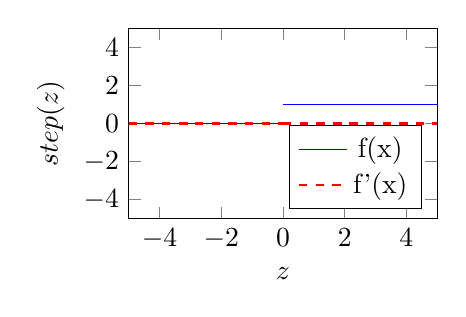
\begin{tikzpicture}
            \begin{axis}
                [width=5.5cm,height=4cm,ylabel=$step(z)$,xlabel=$z$,ymin=-5.0,ymax=5.0,xmin=-5,xmax=5,
                legend style={at={(0.95,0.05)},anchor=south east},]
                \addplot[blue,smooth, domain=-5:0] {0};
                \addplot[red,dashed, thick, domain=-5:0] {0};
                \addplot[blue,smooth, domain=-0:5] {1};
                \addplot[red,dashed, thick, domain=-0:5] {0};
                \addlegendentry{f(x)}
                \addlegendentry{f'(x)}
            \end{axis}
        \end{tikzpicture}
    }
    \subfloat[Linear]{
        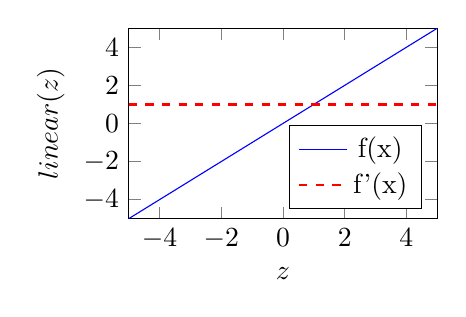
\begin{tikzpicture}
            \begin{axis}
                [width=5.5cm,height=4cm,ylabel=$linear(z)$,xlabel=$z$,ymin=-5.0,ymax=5.0,xmin=-5,xmax=5,
                legend style={at={(0.95,0.05)},anchor=south east},]
                \addplot[blue,smooth] {x};
                \addlegendentry{f(x)}
                \addplot[red,dashed, thick] {1};
                \addlegendentry{f'(x)}
            \end{axis}
        \end{tikzpicture}
    }
    \subfloat[Sigmoid]{
        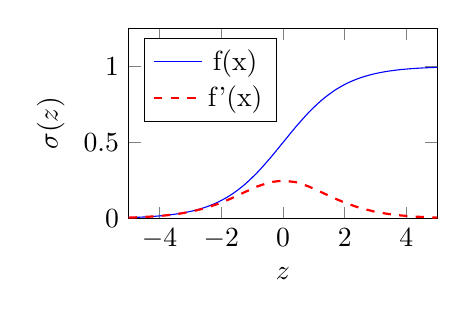
\begin{tikzpicture}
            \begin{axis}
                [width=5.5cm,height=4cm,ylabel=$\sigma(z)$,xlabel=$z$,ymin=0,ymax=1.25,xmin=-5,xmax=5,
                legend style={at={(0.05,0.95)},anchor=north west},]
                \addplot[blue,smooth] {1/(1+exp(-x))};
                \addlegendentry{f(x)}
                \addplot[red, dashed, thick] {1/(1+exp(-x)) * (1-1/(1+exp(-x)))};
                \addlegendentry{f'(x)}
            \end{axis}
        \end{tikzpicture}
    }\\
    \subfloat[Hyperbolic tangent]{
        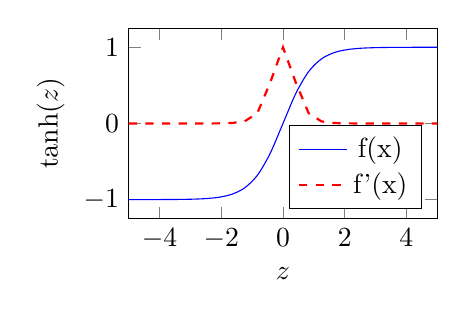
\begin{tikzpicture}
            \begin{axis}
                [width=5.5cm,height=4cm,ylabel=$\tanh(z)$,xlabel=$z$,ymin=-1.25,ymax=1.25,xmin=-5,xmax=5, legend style={at={(0.95,0.05)},anchor=south east},]
                \addplot[blue,smooth] {tanh(x)};
                \addlegendentry{f(x)}
                \addplot[red,dashed, thick] {1/cosh(2*x)*1/cosh(2*x)};
                \addlegendentry{f'(x)}
            \end{axis}
        \end{tikzpicture}
    }
    \subfloat[ReLU]{
        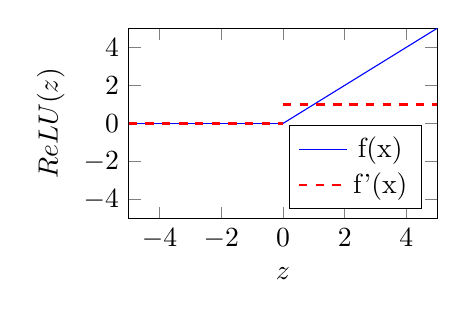
\begin{tikzpicture}
            \begin{axis}
                [width=5.5cm,height=4cm,ylabel=$ReLU(z)$,xlabel=$z$,ymin=-5.0,ymax=5.0,xmin=-5,xmax=5,
                legend style={at={(0.95,0.05)},anchor=south east},]
                \addplot[blue,smooth, domain=-5:0] {0};
                \addplot[red,dashed, thick, domain=-5:0] {0};
                \addplot[blue,smooth, domain=-0:5] {x};
                \addplot[red,dashed, thick, domain=-0:5] {1};
                \addlegendentry{f(x)}
                \addlegendentry{f'(x)}
            \end{axis}
        \end{tikzpicture}
    }
    \subfloat[Leaky ReLU]{
        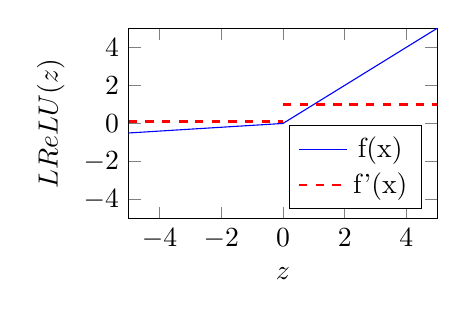
\begin{tikzpicture}
            \begin{axis}
                [width=5.5cm,height=4cm,ylabel=$LReLU(z)$,xlabel=$z$,ymin=-5.0,ymax=5.0,xmin=-5,xmax=5,
                legend style={at={(0.95,0.05)},anchor=south east},]
                \addplot[blue,smooth, domain=-5:0] {0.1*x};
                \addplot[red,dashed, thick, domain=-5:0] {0.1};
                \addplot[blue,smooth, domain=-0:5] {x};
                \addplot[red,dashed, thick, domain=-0:5] {1};
                \addlegendentry{f(x)}
                \addlegendentry{f'(x)}
            \end{axis}
        \end{tikzpicture}
    }\\
    \subfloat[GELU]{
        \begin{tikzpicture}
            \begin{axis}
                [width=5.5cm,height=4cm,ylabel=$GELU(z)$,xlabel=$z$,ymin=-5.0,ymax=5.0,xmin=-5,xmax=5,
                legend style={at={(0.95,0.05)},anchor=south east},]
                \addplot[blue,smooth] {x * 0.5 * (1 + erf(x /sqrt(2)))};
                \addplot[red,dashed, thick] {0.5 * (1 + erf(x /sqrt(2))) + 1/sqrt(2*pi) * (exp(-x*x/2))};
                \addlegendentry{f(x)}
                \addlegendentry{f'(x)}
            \end{axis}
        \end{tikzpicture}
    }
    \subfloat[Swish]{
        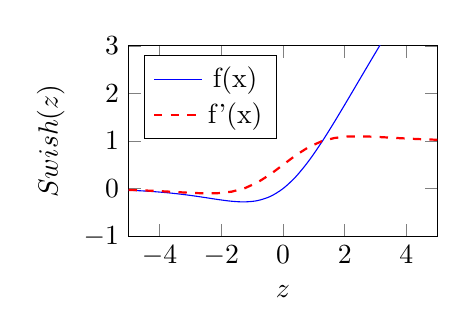
\begin{tikzpicture}
            \begin{axis}
                [width=5.5cm,height=4cm,ylabel=$Swish(z)$,xlabel=$z$,ymin=-1,ymax=3.0,xmin=-5,xmax=5,
                legend style={at={(0.05,0.95)},anchor=north west},]
                \addplot[blue,smooth] {x*(1/(1+exp(-x)))}; % f (x) + σ (x) (1 − f (x))
                \addlegendentry{f(x)}
                \addplot[red, dashed, thick] {x/(1+exp(-x)) + 1/(1+exp(-x)) * (1-x/(1+exp(-x)))};
                \addlegendentry{f'(x)}
            \end{axis}
        \end{tikzpicture}
    }
    \subfloat[]{
        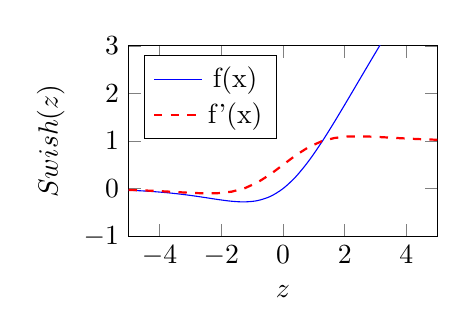
\begin{tikzpicture}
            \begin{axis}
                [width=5.5cm,height=4cm,ylabel=$Swish(z)$,xlabel=$z$,ymin=-1,ymax=3.0,xmin=-5,xmax=5,
                legend style={at={(0.05,0.95)},anchor=north west},]
                \addplot[blue,smooth] {x*(1/(1+exp(-x)))}; % f (x) + σ (x) (1 − f (x))
                \addlegendentry{f(x)}
                \addplot[red, dashed, thick] {x/(1+exp(-x)) + 1/(1+exp(-x)) * (1-x/(1+exp(-x)))};
                \addlegendentry{f'(x)}
            \end{axis}
        \end{tikzpicture}
    }
    \caption[Sigmoidal activation functions.]{Commonly used activation functions in MLPs.}
    \label{fig:activation-functions}
\end{figure}
%    \caption{Activation functions}
%    \label{fig:activation}
%\end{figure}
\makeatletter
\pgfmathdeclarefunction{erf}{1}{%
    \begingroup
    \pgfmathparse{#1 > 0 ? 1 : -1}%
    \edef\sign{\pgfmathresult}%
    \pgfmathparse{abs(#1)}%
    \edef\x{\pgfmathresult}%
    \pgfmathparse{1/(1+0.3275911*\x)}%
    \edef\t{\pgfmathresult}%
    \pgfmathparse{%
        1 - (((((1.061405429*\t -1.453152027)*\t) + 1.421413741)*\t
        -0.284496736)*\t + 0.254829592)*\t*exp(-(\x*\x))}%
    \edef\y{\pgfmathresult}%
    \pgfmathparse{(\sign)*\y}%
    \pgfmath@smuggleone\pgfmathresult%
    \endgroup
}
%dep
%subfig
\begin{figure}[t!]
    \centering
    \subfloat[Threshold Step]{
        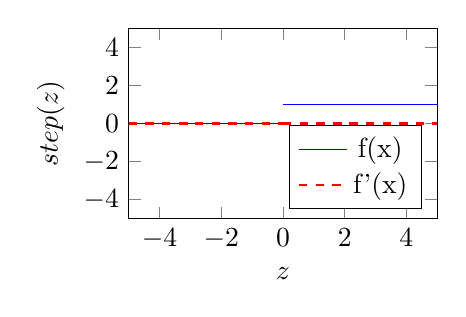
\begin{tikzpicture}
            \begin{axis}
                [width=5.5cm,height=4cm,ylabel=$step(z)$,xlabel=$z$,ymin=-5.0,ymax=5.0,xmin=-5,xmax=5,
                legend style={at={(0.95,0.05)},anchor=south east},]
                \addplot[blue,smooth, domain=-5:0] {0};
                \addplot[red,dashed, thick, domain=-5:0] {0};
                \addplot[blue,smooth, domain=-0:5] {1};
                \addplot[red,dashed, thick, domain=-0:5] {0};
                \addlegendentry{f(x)}
                \addlegendentry{f'(x)}
            \end{axis}
        \end{tikzpicture}
    }
    \subfloat[Linear]{
        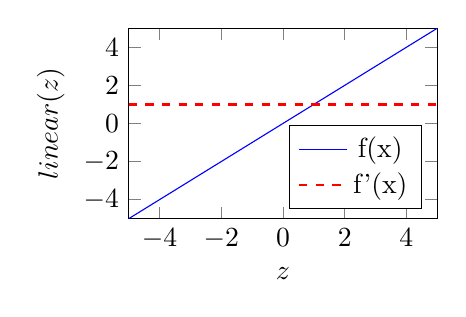
\begin{tikzpicture}
            \begin{axis}
                [width=5.5cm,height=4cm,ylabel=$linear(z)$,xlabel=$z$,ymin=-5.0,ymax=5.0,xmin=-5,xmax=5,
                legend style={at={(0.95,0.05)},anchor=south east},]
                \addplot[blue,smooth] {x};
                \addlegendentry{f(x)}
                \addplot[red,dashed, thick] {1};
                \addlegendentry{f'(x)}
            \end{axis}
        \end{tikzpicture}
    }
    \subfloat[Sigmoid]{
        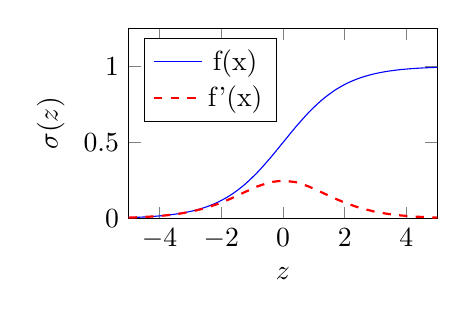
\begin{tikzpicture}
            \begin{axis}
                [width=5.5cm,height=4cm,ylabel=$\sigma(z)$,xlabel=$z$,ymin=0,ymax=1.25,xmin=-5,xmax=5,
                legend style={at={(0.05,0.95)},anchor=north west},]
                \addplot[blue,smooth] {1/(1+exp(-x))};
                \addlegendentry{f(x)}
                \addplot[red, dashed, thick] {1/(1+exp(-x)) * (1-1/(1+exp(-x)))};
                \addlegendentry{f'(x)}
            \end{axis}
        \end{tikzpicture}
    }\\
    \subfloat[Hyperbolic tangent]{
        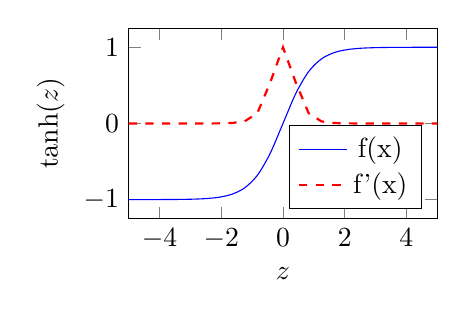
\begin{tikzpicture}
            \begin{axis}
                [width=5.5cm,height=4cm,ylabel=$\tanh(z)$,xlabel=$z$,ymin=-1.25,ymax=1.25,xmin=-5,xmax=5, legend style={at={(0.95,0.05)},anchor=south east},]
                \addplot[blue,smooth] {tanh(x)};
                \addlegendentry{f(x)}
                \addplot[red,dashed, thick] {1/cosh(2*x)*1/cosh(2*x)};
                \addlegendentry{f'(x)}
            \end{axis}
        \end{tikzpicture}
    }
    \subfloat[ReLU]{
        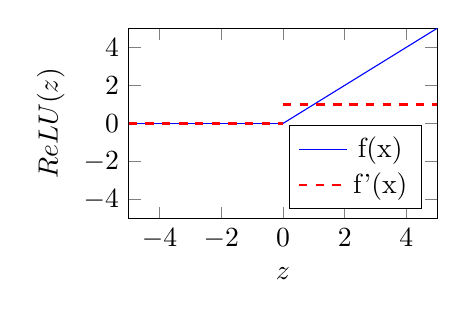
\begin{tikzpicture}
            \begin{axis}
                [width=5.5cm,height=4cm,ylabel=$ReLU(z)$,xlabel=$z$,ymin=-5.0,ymax=5.0,xmin=-5,xmax=5,
                legend style={at={(0.95,0.05)},anchor=south east},]
                \addplot[blue,smooth, domain=-5:0] {0};
                \addplot[red,dashed, thick, domain=-5:0] {0};
                \addplot[blue,smooth, domain=-0:5] {x};
                \addplot[red,dashed, thick, domain=-0:5] {1};
                \addlegendentry{f(x)}
                \addlegendentry{f'(x)}
            \end{axis}
        \end{tikzpicture}
    }
    \subfloat[Leaky ReLU]{
        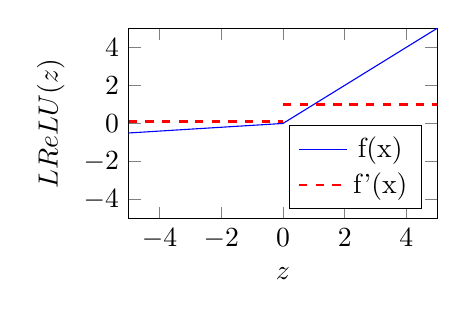
\begin{tikzpicture}
            \begin{axis}
                [width=5.5cm,height=4cm,ylabel=$LReLU(z)$,xlabel=$z$,ymin=-5.0,ymax=5.0,xmin=-5,xmax=5,
                legend style={at={(0.95,0.05)},anchor=south east},]
                \addplot[blue,smooth, domain=-5:0] {0.1*x};
                \addplot[red,dashed, thick, domain=-5:0] {0.1};
                \addplot[blue,smooth, domain=-0:5] {x};
                \addplot[red,dashed, thick, domain=-0:5] {1};
                \addlegendentry{f(x)}
                \addlegendentry{f'(x)}
            \end{axis}
        \end{tikzpicture}
    }\\
    \subfloat[GELU]{
        \begin{tikzpicture}
            \begin{axis}
                [width=5.5cm,height=4cm,ylabel=$GELU(z)$,xlabel=$z$,ymin=-5.0,ymax=5.0,xmin=-5,xmax=5,
                legend style={at={(0.95,0.05)},anchor=south east},]
                \addplot[blue,smooth] {x * 0.5 * (1 + erf(x /sqrt(2)))};
                \addplot[red,dashed, thick] {0.5 * (1 + erf(x /sqrt(2))) + 1/sqrt(2*pi) * (exp(-x*x/2))};
                \addlegendentry{f(x)}
                \addlegendentry{f'(x)}
            \end{axis}
        \end{tikzpicture}
    }
    \subfloat[Swish]{
        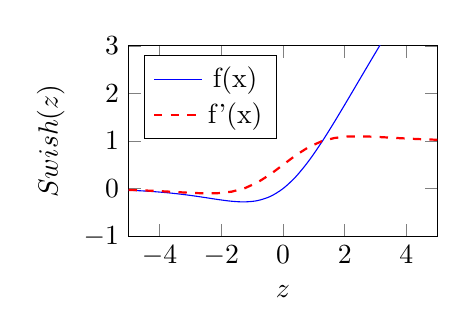
\begin{tikzpicture}
            \begin{axis}
                [width=5.5cm,height=4cm,ylabel=$Swish(z)$,xlabel=$z$,ymin=-1,ymax=3.0,xmin=-5,xmax=5,
                legend style={at={(0.05,0.95)},anchor=north west},]
                \addplot[blue,smooth] {x*(1/(1+exp(-x)))}; % f (x) + σ (x) (1 − f (x))
                \addlegendentry{f(x)}
                \addplot[red, dashed, thick] {x/(1+exp(-x)) + 1/(1+exp(-x)) * (1-x/(1+exp(-x)))};
                \addlegendentry{f'(x)}
            \end{axis}
        \end{tikzpicture}
    }
    \subfloat[]{
        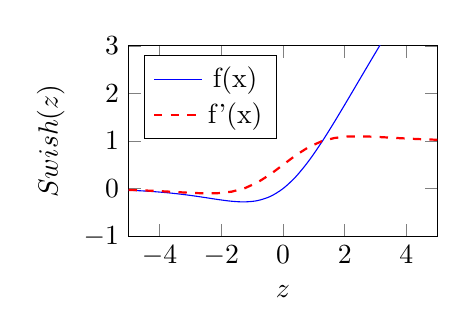
\begin{tikzpicture}
            \begin{axis}
                [width=5.5cm,height=4cm,ylabel=$Swish(z)$,xlabel=$z$,ymin=-1,ymax=3.0,xmin=-5,xmax=5,
                legend style={at={(0.05,0.95)},anchor=north west},]
                \addplot[blue,smooth] {x*(1/(1+exp(-x)))}; % f (x) + σ (x) (1 − f (x))
                \addlegendentry{f(x)}
                \addplot[red, dashed, thick] {x/(1+exp(-x)) + 1/(1+exp(-x)) * (1-x/(1+exp(-x)))};
                \addlegendentry{f'(x)}
            \end{axis}
        \end{tikzpicture}
    }
    \caption[Sigmoidal activation functions.]{Commonly used activation functions in MLPs.}
    \label{fig:activation-functions}
\end{figure}

\subsection{Multi-layer perceptrons}
%%%%%%%%%%%%%%%%%%%%%%%%%%%%%%%%%%%%%%%%%%%%%%%%%%%%%%%%%%%%%%%%%%%%%%%%%%%%%%%%
\Gls{MLPs}, otherwise known as \textbf{artificial neural networks} or
\textbf{feedforward neural networks}, are the fundamental models of \gls{DL}.
They adapt and

\textbf{Deep feedforward networks}
\\
$f(\gls{x_in}; \gls{theta})$; $\gls{x_in}\in\mathbb{R}^{\gls{n_x}}$

\begin{figure}
    \centering
    % MIT License
%
% Copyright (c) 2021 Geoffrey H. Garrett
%
% Permission is hereby granted, free of charge, to any person obtaining a copy
% of this software and associated documentation files (the "Software"), to deal
% in the Software without restriction, including without limitation the rights
% to use, copy, modify, merge, publish, distribute, sublicense, and/or sell
% copies of the Software, and to permit persons to whom the Software is
% furnished to do so, subject to the following conditions:
%
% The above copyright notice and this permission notice shall be included in all
% copies or substantial portions of the Software.
%
% THE SOFTWARE IS PROVIDED "AS IS", WITHOUT WARRANTY OF ANY KIND, EXPRESS OR
% IMPLIED, INCLUDING BUT NOT LIMITED TO THE WARRANTIES OF MERCHANTABILITY,
% FITNESS FOR A PARTICULAR PURPOSE AND NONINFRINGEMENT. IN NO EVENT SHALL THE
% AUTHORS OR COPYRIGHT HOLDERS BE LIABLE FOR ANY CLAIM, DAMAGES OR OTHER
% LIABILITY, WHETHER IN AN ACTION OF CONTRACT, TORT OR OTHERWISE, ARISING FROM,
% OUT OF OR IN CONNECTION WITH THE SOFTWARE OR THE USE OR OTHER DEALINGS IN THE
% SOFTWARE.

%%%%%%%%%%%%%%%%%%%%%%%%%%%%%%%%%%%%%%%%%%%%%%%%%%%%%%%%%%%%%%%%%%%%%%%%%%%%%%%
% ACKNOWLEDGEMENTS
%%%%%%%%%%%%%%%%%%%%%%%%%%%%%%%%%%%%%%%%%%%%%%%%%%%%%%%%%%%%%%%%%%%%%%%%%%%%%%%
% Adapted from:
% https://www.researchgate.net/figure/The-agent-environment-interaction-in-reinforcement-learning_fig1_328494763

%%%%%%%%%%%%%%%%%%%%%%%%%%%%%%%%%%%%%%%%%%%%%%%%%%%%%%%%%%%%%%%%%%%%%%%%%%%%%%%
% DEPENDENCIES
%%%%%%%%%%%%%%%%%%%%%%%%%%%%%%%%%%%%%%%%%%%%%%%%%%%%%%%%%%%%%%%%%%%%%%%%%%%%%%%
%\usepackage{tikz}
%\usetikzlibrary{decorations.pathreplacing}    % for TikZ braces
%\usetikzlibrary{positioning}                  % for TikZ relative positioning

%%%%%%%%%%%%%%%%%%%%%%%%%%%%%%%%%%%%%%%%%%%%%%%%%%%%%%%%%%%%%%%%%%%%%%%%%%%%%%%
% USER STYLING
%%%%%%%%%%%%%%%%%%%%%%%%%%%%%%%%%%%%%%%%%%%%%%%%%%%%%%%%%%%%%%%%%%%%%%%%%%%%%%%

% TikZ node design.
\tikzset{basic/.style={draw,text width=1em,text badly centered}}
\tikzset{input/.style={basic, fill=green!25, circle}}
\tikzset{output/.style={basic, fill=blue!25, circle}}
\tikzset{weight/.style={basic,circle}}
\tikzset{hidden/.style={basic,circle}}
\tikzset{function/.style={basic,circle}}
\def\layersep{3em}
\def\transferx{9em}
\def\hiddenx{7em}
\def\hiddenxn{12em}


\def\sep{4em}
\def\L{\gls{L}}       % number of hidden layers
\def\y{\gls{y_true}}  % output vector
\def\x{\gls{ml:x}}    % input vector
\def\h{\gls{a_vec}}   % hidden output
\def\nx{\gls{ml:n_x}}   % hidden output
\def\ny{\gls{ml:n_y}}   % hidden output


%%%%%%%%%%%%%%%%%%%%%%%%%%%%%%%%%%%%%%%%%%%%%%%%%%%%%%%%%%%%%%%%%%%%%%%%%%%%%%%
% TIKZ PICTURE
%%%%%%%%%%%%%%%%%%%%%%%%%%%%%%%%%%%%%%%%%%%%%%%%%%%%%%%%%%%%%%%%%%%%%%%%%%%%%%%
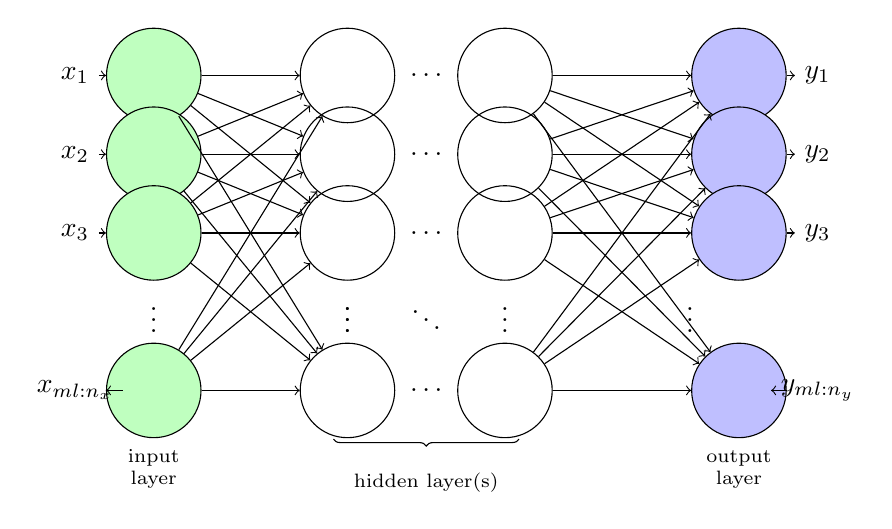
\begin{tikzpicture}
    \usetikzlibrary{decorations.pathreplacing}    % for TikZ braces
    \usetikzlibrary{positioning}                  % for TikZ relative positioning

    % input
    \foreach \n/\p in {0/1,1/2,2/3,3/4,4/5} {
        \ifnum \n=3
            % dots layer
            \node[] at (0, -\n) (X_\n) {$\vdots$};
            \node[] at (\hiddenx, -\n) (H1_\n) {$\vdots$};
            \node[right of=H1_\n] (M-\n) {$\ddots$};
            \node[below of=H1_2] (H2_\n) {$\vdots$};
            \node[below of=H2_2] (H2_\n) {$\vdots$};
            \node[right=5.7em of H2_\n] (Y_\n) {$\vdots$};
        \else
        \ifnum \n=4
            % n layer
            \node[input] at (0, -\n) (X_\n) {};
            \node[left of=X_\n] (I_\n) {$x_{\nx}$};
            \path[draw,->] (I_\n) -- (X_\n);
            \node[hidden] at (\hiddenx, -\n) (H1_\n) {}; %{$h_{n, 1}$};
            \node[right of= H1_\n] (M-\n) {$\ldots$};
            \node[hidden, right of= M-\n] (H2_\n) {}; % {$h_{n, m}$};
            \node[output, right= 5em of H2_\n] (Y_\n) {}; % {$h_{n, m}$};
            \node[right of=Y_\n] (O_\n) {$y_{\ny}$};
            \path[draw,->] (Y_\n) -- (O_\n);
        \else
            \node[input] at (0, -{\n}) (X_\n) {};
            \node[left of=X_\n] (I_\n) {$x_{\p}$};
            \path[draw,->] (I_\n) -- (X_\n);
            \node[hidden] at (\hiddenx, -\n) (H1_\n) {};%{$h_{\n, 1}$};
            \node[right of=H1_\n] (M-\n) {$\ldots$};
            \node[hidden, right of=M-\n] (H2_\n) {};% {$h_{\n, m}$};
            \node[output, right= 5em of H2_\n] (Y_\n) {}; % {$h_{n, m}$};
            \node[right of=Y_\n] (O_\n) {$y_\p$};
            \path[draw,->] (Y_\n) -- (O_\n);
        \fi
        \fi
    }

    % input layer connected to first hidden layer
    \foreach \j in {0,1,2,4} {
        \foreach \n in {0,1,2,4} {
            \path[draw,->] (X_\n) -- (H1_\j);
        }
    }

    % second hidden layer connected to output layer
    \foreach \j in {0,1,2,4} {
        \foreach \n in {0,1,2,4} {
            \path[draw,->] (H2_\n) -- (Y_\j);
        }
    }

    % labels
    \node[below of=X_4,font=\scriptsize, align=center] {input\\layer};
    \node[below of=Y_4,font=\scriptsize, align=center] {output\\layer};

    % brace for hidden layers
    \node[below=1em of M-4] (hidden-brace) {};
    \node[right=3em of hidden-brace] (hidden-brace-right) {};
    \node[left=3em of hidden-brace] (hidden-brace-left) {};
    \draw [decorate,decoration = {brace}] (hidden-brace-right) --  (hidden-brace-left);
    \node[below=0.5em of hidden-brace,font=\scriptsize] (hlayer) {hidden layer(s)};

\end{tikzpicture}


    \caption{Multilayer perceptron}
    \label{fig:mlp}
\end{figure}


\begin{figure}
    \centering
    % MIT License
%
% Copyright (c) 2021 Geoffrey H. Garrett
%
% Permission is hereby granted, free of charge, to any person obtaining a copy
% of this software and associated documentation files (the "Software"), to deal
% in the Software without restriction, including without limitation the rights
% to use, copy, modify, merge, publish, distribute, sublicense, and/or sell
% copies of the Software, and to permit persons to whom the Software is
% furnished to do so, subject to the following conditions:
%
% The above copyright notice and this permission notice shall be included in all
% copies or substantial portions of the Software.
%
% THE SOFTWARE IS PROVIDED "AS IS", WITHOUT WARRANTY OF ANY KIND, EXPRESS OR
% IMPLIED, INCLUDING BUT NOT LIMITED TO THE WARRANTIES OF MERCHANTABILITY,
% FITNESS FOR A PARTICULAR PURPOSE AND NONINFRINGEMENT. IN NO EVENT SHALL THE
% AUTHORS OR COPYRIGHT HOLDERS BE LIABLE FOR ANY CLAIM, DAMAGES OR OTHER
% LIABILITY, WHETHER IN AN ACTION OF CONTRACT, TORT OR OTHERWISE, ARISING FROM,
% OUT OF OR IN CONNECTION WITH THE SOFTWARE OR THE USE OR OTHER DEALINGS IN THE
% SOFTWARE.

%%%%%%%%%%%%%%%%%%%%%%%%%%%%%%%%%%%%%%%%%%%%%%%%%%%%%%%%%%%%%%%%%%%%%%%%%%%%%%%
% DEPENDENCIES
%%%%%%%%%%%%%%%%%%%%%%%%%%%%%%%%%%%%%%%%%%%%%%%%%%%%%%%%%%%%%%%%%%%%%%%%%%%%%%%
%\usepackage{tikz}
%\usetikzlibrary{decorations.pathreplacing}    % for TikZ braces
%\usetikzlibrary{positioning}                  % for TikZ relative positioning

%%%%%%%%%%%%%%%%%%%%%%%%%%%%%%%%%%%%%%%%%%%%%%%%%%%%%%%%%%%%%%%%%%%%%%%%%%%%%%%
% USER STYLING
%%%%%%%%%%%%%%%%%%%%%%%%%%%%%%%%%%%%%%%%%%%%%%%%%%%%%%%%%%%%%%%%%%%%%%%%%%%%%%%

% TikZ node design.
\tikzset{basic/.style={draw,text badly centered}}
\tikzset{input/.style={basic,minimum width=1.2cm, fill=green!25, circle}}
\tikzset{output/.style={basic,minimum width=1.2cm, fill=blue!25, circle}}
\tikzset{weight/.style={basic,circle}}
\tikzset{hidden/.style={basic,circle, minimum width=1.2cm}}
\tikzset{function/.style={basic,circle}}

\def\sep{4em}
\def\L{\gls{L}}       % number of hidden layers
\def\y{\gls{y_pred}}  % output vector
\def\x{\gls{ml:x}}    % input vector
\def\h{\gls{a_vec}}   % hidden output

%%%%%%%%%%%%%%%%%%%%%%%%%%%%%%%%%%%%%%%%%%%%%%%%%%%%%%%%%%%%%%%%%%%%%%%%%%%%%%%
% TIKZ PICTURE
%%%%%%%%%%%%%%%%%%%%%%%%%%%%%%%%%%%%%%%%%%%%%%%%%%%%%%%%%%%%%%%%%%%%%%%%%%%%%%%
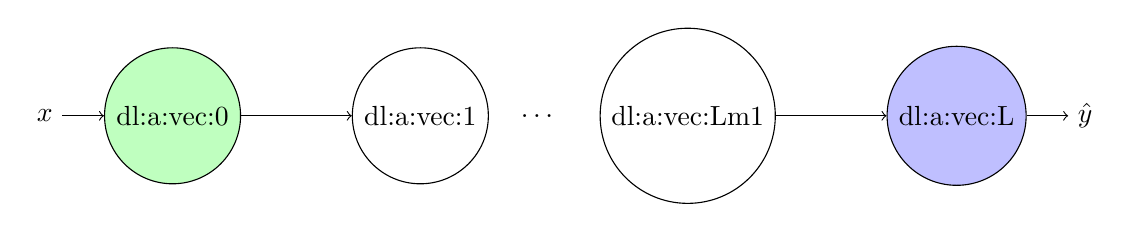
\begin{tikzpicture}
    \node[input, label={[xshift=-0.0em]center:\gls{dl:a:vec:0}}] (X) {\phantom{\gls{dl:a:vec:1}}};
    \node[, left=1.5em of X] (in) {$\bm{x}$};

    \node[hidden, right=\sep of X, label={[xshift=-0.0em]center:\gls{dl:a:vec:1}}] (H1) {\phantom{\gls{dl:a:vec:1}}};
    \node[hidden, right=\sep of H1, label={[xshift=-0.0em]center:\gls{dl:a:vec:Lm1}}] (H2) {\phantom{\gls{dl:a:vec:Lm1}}};
    \node[output, right=\sep of H2,  label={[xshift=-0.0em]center:\gls{dl:a:vec:L}}] (Y) {\phantom{\gls{dl:a:vec:L}}};
    \node[, right=1.5em of Y] (out) {$\bm{\hat{y}}$};

    \path[draw,->] (in) -- (X);
    \path[draw,->] (X) -- (H1);
    \node[right=0.8em of H1] (M) {$\ldots$};
    \path[draw,->] (H2) -- (Y);
    \path[draw,->] (Y) -- (out);
\end{tikzpicture}


    \caption{Multilayer perceptron}
    \label{fig:mlp-vec}
\end{figure}



\begin{equation}
    \mathbf{a}^{[1]} = g^{[1]} \bigg(\gls{dl:W:1}^T\gls{x_in} + \mathbf{b}^{[1]}\bigg);
\end{equation}

\begin{equation}
    \mathbf{a}^{[2]} = g^{[2]} \bigg(\gls{dl:W:2}^T\mathbf{h}^{[2]} + \mathbf{b}^{[2]}\bigg);
\end{equation}

\gls{dl:W:l}

\subsection{Gradient based learning}
%%%%%%%%%%%%%%%%%%%%%%%%%%%%%%%%%%%%%%%%%%%%%%%%%%%%%%%%%%%%%%%%%%%%%%%%%%%%%%%%

Backpropagation, short for "backward propagation of errors," is a
\textit{supervised learning} algorithm for artificial neural networks using
\textit{gradient descent}.

\begin{figure}[htp]
    \centering
    \input{graphics/tikz/gradient-descent}
    \caption{Gradient based learning}
    \label{fig:gradient-descent}
\end{figure}


\begin{figure}[htp]
    \centering
    \input{graphics/tikz/gradient-descent-3d}
    \caption{Gradient based learning}
    \label{fig:gradient-descent}
\end{figure}

\subsection{Universal Approximation Properties and Depth}
%%%%%%%%%%%%%%%%%%%%%%%%%%%%%%%%%%%%%%%%%%%%%%%%%%%%%%%%%%%%%%%%%%%%%%%%%%%%%%%%

A linear model by definition, may only optimised to represent linear functions.
It has advantages in its simplicity to optimise however we often require our
estimator models to learn nonlinear functions.

%\subsection{Backpropagation}
%%%%%%%%%%%%%%%%%%%%%%%%%%%%%%%%%%%%%%%%%%%%%%%%%%%%%%%%%%%%%%%%%%%%%%%%%%%%%%%%


